\documentclass[11pt]{article}
\usepackage[margin=1in]{geometry}
\usepackage{amsmath,amssymb,amsthm,mathtools}
\usepackage{hyperref}
\usepackage{enumitem}
\usepackage{tikz}
\usetikzlibrary{arrows.meta,positioning}

% --- Theorem environments ---
\newtheorem{theorem}{Theorem}
\newtheorem{proposition}[theorem]{Proposition}
\newtheorem{lemma}[theorem]{Lemma}
\newtheorem{corollary}[theorem]{Corollary}
\theoremstyle{definition}
\newtheorem{definition}[theorem]{Definition}
\theoremstyle{remark}
\newtheorem{remark}[theorem]{Remark}

% --- Notation ---
\newcommand{\R}{\mathbb R}
\newcommand{\1}{\mathbf 1}
\newcommand{\Id}{\mathrm{Id}}
\newcommand{\STD}{\textnormal{\textbf{(Standard)}}}
\newcommand{\NEW}{\textnormal{\textbf{(New presentation)}}}


\title{A Five-Step Energy-Decomposition Proof of the Discrete Dirichlet Ground State Theorem}
\author{}
\date{}

\begin{document}
\maketitle

\begin{abstract}
We give a completely rigorous and undergraduate-accessible proof of the classical ``ground state'' theorem
for the Dirichlet graph Laplacian: on a connected interior, the smallest Dirichlet eigenvalue is simple and admits
a strictly positive eigenfunction on the interior. The proof is organized to mirror a general methodology used in
Dirichlet form theory: (1) energy decomposition, (2) Markov property, (3) irreducibility (connectivity of the interior),
(4) compact resolvent (finite-dimensional), and (5) Perron--Frobenius/Krein--Rutman for a positive compact operator.
Every step is proved concretely for finite graphs.
\end{abstract}

\noindent\textbf{About standardness.}
We label each stated result as \STD\ when it is a well-known statement from linear algebra, spectral graph theory, discrete maximum principles, or Perron--Frobenius theory, and as \NEW\ when the content is primarily expository (e.g., the five-step organization or packaging of several standard facts).
Proofs are included even for \STD\ results when they are short and illuminating.


\tableofcontents

\section{The five-step spine and the main theorem}

\subsection{Flowchart}
\begin{center}
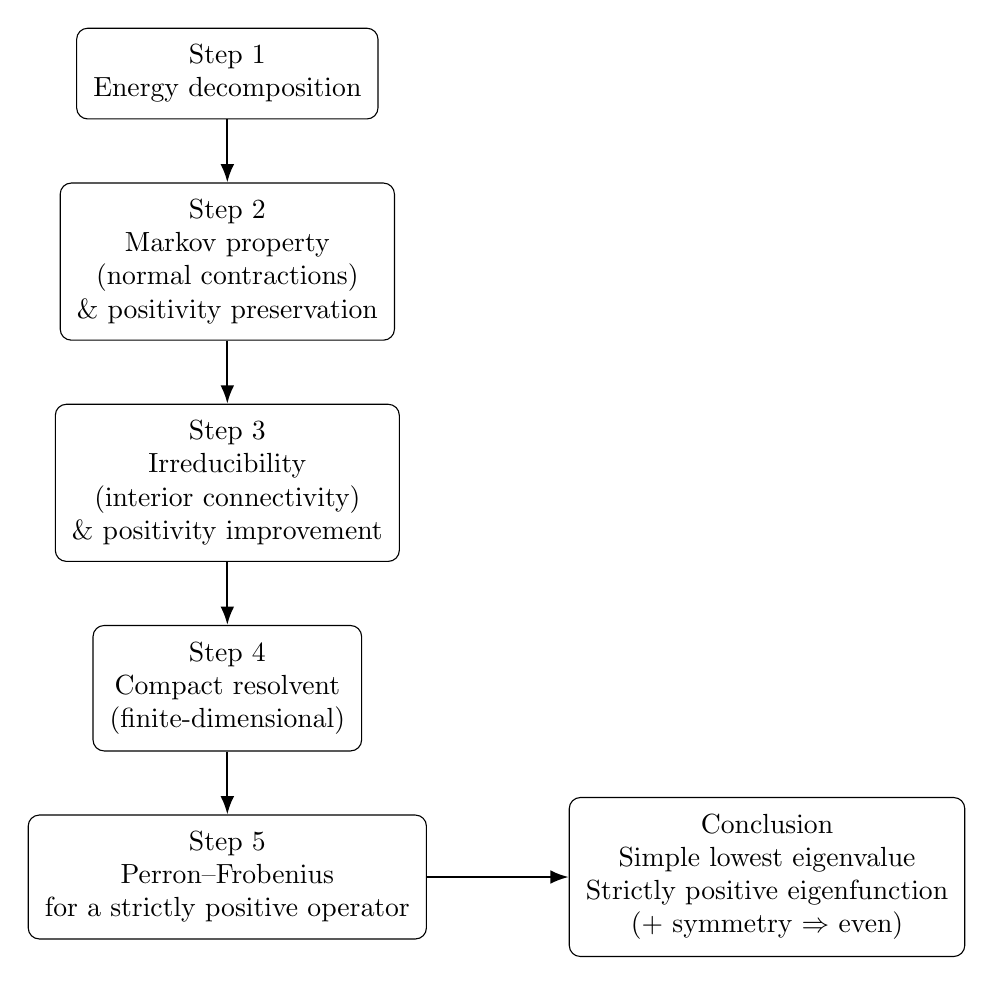
\begin{tikzpicture}[
  node distance=8mm,
  box/.style={draw, rounded corners, align=center, inner sep=6pt},
  arr/.style={-Latex, thick}
]
\node[box] (s1) {Step 1\\Energy decomposition};
\node[box, below=of s1] (s2) {Step 2\\Markov property\\(normal contractions)\\\& positivity preservation};
\node[box, below=of s2] (s3) {Step 3\\Irreducibility\\(interior connectivity)\\\& positivity improvement};
\node[box, below=of s3] (s4) {Step 4\\Compact resolvent\\(finite-dimensional)};
\node[box, below=of s4] (s5) {Step 5\\Perron--Frobenius\\for a strictly positive operator};

\draw[arr] (s1) -- (s2);
\draw[arr] (s2) -- (s3);
\draw[arr] (s3) -- (s4);
\draw[arr] (s4) -- (s5);

\node[box, right=18mm of s5] (out) {Conclusion\\Simple lowest eigenvalue\\Strictly positive eigenfunction\\(+ symmetry $\Rightarrow$ even)};
\draw[arr] (s5.east) -- (out.west);
\end{tikzpicture}
\end{center}

\subsection{Main statement}

\begin{definition}[Weighted graph with boundary and connected interior]\label{def:graph}
Let $G=(V,E,w)$ be a finite undirected graph with vertex set $V$, edge set
$E\subseteq \{\{x,y\}:x\neq y\}$, and weights $w_{xy}=w_{yx}>0$ for $\{x,y\}\in E$
(and $w_{xy}=0$ otherwise).
Fix a nonempty boundary set $B\subset V$, and write $I:=V\setminus B$ for the interior.
Assume:
\begin{enumerate}[label=(\roman*)]
\item $G$ is connected (as an undirected graph),
\item $B\neq \emptyset$ and $I\neq \emptyset$,
\item the \emph{interior induced graph} $G_I:=(I,E_I,w)$ is connected, where
\[
E_I:=\bigl\{\{x,y\}\in E:\ x\in I,\ y\in I\bigr\}.
\]
\end{enumerate}
\end{definition}

\begin{remark}[Why interior connectivity is the right hypothesis]\label{rem:why-interior}
If $G_I$ is not connected, then the Dirichlet operator $L_B$ on $\R^I$ decomposes into a direct sum over the
connected components of $G_I$, and the global smallest eigenvalue need not be simple. In particular, the conclusion
``$\varphi_1>0$ on all of $I$'' can fail. Theorem \ref{thm:main} therefore assumes the standard analogue of
``connected domain'': connectivity of the interior.
A fully general componentwise statement is recorded in Remark \ref{rem:componentwise} below.
\end{remark}

\begin{definition}[Dirichlet Laplacian]\label{def:dirichletL}
For a function $f:V\to\R$ with $f|_B=0$, define for $x\in I$
\begin{equation}\label{eq:dirichletL}
(L_B f)(x) := \sum_{y\in V} w_{xy}\,\bigl(f(x)-f(y)\bigr),
\end{equation}
where $f(y)=0$ for $y\in B$ (Dirichlet condition).
Equivalently, $L_B$ is the principal submatrix of the full Laplacian corresponding to $I$.
We view $L_B$ as a linear operator on $\R^I$ by identifying $f\in\R^I$ with its zero extension to $V$.
\end{definition}

\begin{theorem}[Discrete Dirichlet ground state theorem \STD]\label{thm:main}
Let $(G,w)$ be a finite connected weighted graph and $B\subset V$ be a nonempty boundary set, with interior
$I=V\setminus B$ nonempty, and assume the induced interior graph $G_I$ is connected.
Then:
\begin{enumerate}[label=(\alph*)]
\item The smallest eigenvalue $\lambda_1$ of $L_B$ (acting on $\R^I$) is strictly positive.
\item $\lambda_1$ is simple (geometric and algebraic multiplicity one).
\item An eigenfunction $\varphi_1$ for $\lambda_1$ can be chosen strictly positive on $I$:
\[
\varphi_1(x)>0\quad\text{for all }x\in I.
\]
\item (Optional symmetry corollary) If $R:V\to V$ is an involution ($R^2=\mathrm{id}$) preserving $E,w$ and preserving $B$,
then $\varphi_1$ can be chosen $R$-even: $\varphi_1\circ R=\varphi_1$ on $I$.
\end{enumerate}
\end{theorem}

\begin{remark}[What is ``known'' versus what is ``methodology'' \NEW]
Theorem \ref{thm:main} is classical in spectral graph theory (see, e.g., \cite{Chung,BiyikogluLeydoldStadler}); what is emphasized here is the organization into the five-step
energy-decomposition spine and the explicit, reusable pattern of the proof.
\end{remark}

\section{Step 0: The Dirichlet energy form and the variational viewpoint}

We work in the finite-dimensional Hilbert space $\ell^2(I)$ with inner product
$\langle f,g\rangle := \sum_{x\in I} f(x)g(x)$.

\begin{definition}[Dirichlet energy form]\label{def:energy}
For $f,g\in\R^I$, let $\tilde f,\tilde g:V\to\R$ be their zero extensions: $\tilde f|_I=f$ and $\tilde f|_B=0$.
Define the symmetric bilinear form
\begin{equation}\label{eq:Efg}
\mathcal E(f,g) := \frac12\sum_{\{x,y\}\in E} w_{xy}\,\bigl(\tilde f(x)-\tilde f(y)\bigr)\bigl(\tilde g(x)-\tilde g(y)\bigr),
\end{equation}
and write $\mathcal E(f):=\mathcal E(f,f)$.
\end{definition}

\begin{lemma}[Green's identity: the generator of the form \STD]\label{lem:greens}
For all $f,g\in\R^I$,
\[
\mathcal E(f,g)=\langle L_B f, g\rangle.
\]
In particular, $L_B$ is self-adjoint and positive semidefinite.
\end{lemma}

\begin{proof}
Write $f,g$ for their zero extensions on $V$ to simplify notation. Expand:
\[
\mathcal E(f,g)=\frac12\sum_{\{x,y\}\in E} w_{xy}\,(f(x)-f(y))(g(x)-g(y)).
\]
Regroup by vertices $x\in I$ (note $g|_B=0$):
\[
\mathcal E(f,g)
=\sum_{x\in I} g(x)\sum_{y\in V} w_{xy}(f(x)-f(y))
=\sum_{x\in I} g(x)\,(L_B f)(x)
=\langle L_B f,g\rangle.
\]
Self-adjointness follows by symmetry of $\mathcal E$, and $\mathcal E(f)=\langle L_B f,f\rangle\ge 0$ gives positivity.
\end{proof}

\begin{remark}[Background: spectral theorem for symmetric matrices \STD]\label{rem:spectral}
We repeatedly use that real symmetric matrices have an orthonormal eigenbasis and real eigenvalues (the spectral theorem);
see, e.g., \cite{Axler,HornJohnson}.
\end{remark}

\begin{remark}[Variational characterization (optional background)]
Since $L_B$ is real symmetric, its eigenvalues are real and its smallest eigenvalue satisfies
\[
\lambda_1 = \min_{f\neq 0}\frac{\langle L_B f,f\rangle}{\langle f,f\rangle}
= \min_{f\neq 0}\frac{\mathcal E(f)}{\|f\|_2^2}.
\]
We will not use calculus of variations for the positivity/simplicity conclusions; instead we follow the five-step spine.
\end{remark}

\section{Step 1: Energy decomposition}

\begin{proposition}[Energy decomposition \STD]\label{prop:decomp}
For every $f\in\R^I$,
\begin{equation}\label{eq:edgedecomp}
\mathcal E(f)=\frac12\sum_{\{x,y\}\in E} w_{xy}\,\bigl(\tilde f(x)-\tilde f(y)\bigr)^2.
\end{equation}
In particular, $\mathcal E(f)=0$ if and only if $\tilde f(x)=\tilde f(y)$ for every edge $\{x,y\}\in E$.
\end{proposition}

\begin{proof}
This is immediate from Definition \ref{def:energy} with $g=f$, and each summand is nonnegative.
\end{proof}

\section{Step 2: Markov property (normal contractions) and positivity preservation}

\begin{definition}[Normal contraction]
A function $\Phi:\R\to\R$ is a \emph{normal contraction} if $\Phi(0)=0$ and
\[
|\Phi(a)-\Phi(b)|\le |a-b|\quad \text{for all }a,b\in\R.
\]
\end{definition}

\begin{lemma}[Markov property \STD]\label{lem:markov}
For any normal contraction $\Phi$ and any $f\in\R^I$,
\[
\mathcal E(\Phi\circ f)\le \mathcal E(f),
\]
where $(\Phi\circ f)(x):=\Phi(f(x))$ on $I$ and is extended by $0$ on $B$ (consistent with $\Phi(0)=0$).
\end{lemma}

\begin{proof}
For each edge $\{x,y\}\in E$,
\[
\bigl(\Phi(\tilde f(x))-\Phi(\tilde f(y))\bigr)^2 \le \bigl(\tilde f(x)-\tilde f(y)\bigr)^2
\]
by the 1-Lipschitz property. Multiply by $w_{xy}$, sum over edges, and use \eqref{eq:edgedecomp}.
\end{proof}

\begin{remark}[How Step 2 is used \NEW]\label{rem:step2use}
Lemma \ref{lem:markov} is a standard ``Markovianity'' property of the Dirichlet form
(see, e.g., \cite{FukushimaOshimaTakeda,BiyikogluLeydoldStadler} for general Dirichlet forms and for graph Laplacians).
In the present finite-graph proof, we will not use Lemma \ref{lem:markov} directly; instead we use the closely related and
equally standard consequence that the resolvent $(L_B+\mu\Id)^{-1}$ is positivity preserving (Lemma \ref{lem:resolvent-positive}).
\end{remark}

\begin{definition}[Positive and negative parts]
For $u\in\R^I$, define $u^+(x):=\max\{u(x),0\}$ and $u^-(x):=\max\{-u(x),0\}$ so that $u=u^+-u^-$ and $u^+u^-=0$ pointwise.
\end{definition}

\begin{lemma}[Scalar inequality for the negative part \STD]\label{lem:scalarineq}
For all $a,b\in\R$, writing $t^-:=\max\{-t,0\}$, one has
\begin{equation}\label{eq:scalar-monotone}
(a-b)\bigl(a^- - b^-\bigr)\le -\bigl(a^- - b^-\bigr)^2.
\end{equation}
\end{lemma}

\begin{proof}
We distinguish cases.
\begin{enumerate}[label=(\roman*)]
\item If $a\ge 0$ and $b\ge 0$, then $a^-=b^-=0$, so both sides are $0$.
\item If $a\le 0$ and $b\le 0$, then $a^-=-a$ and $b^-=-b$, so the left-hand side equals
\[
(a-b)\bigl((-a)-(-b)\bigr)=(a-b)(-a+b)=-(a-b)^2=-(a^--b^-)^2.
\]
\item If $a\ge 0$ and $b\le 0$, then $a^-=0$ and $b^-=-b$, so $a^- - b^-=b$ and
\[
(a-b)(a^- - b^-)= (a-b)b = ab-b^2 \le -b^2=-(a^- - b^-)^2,
\]
since $ab\le 0$. The case $a\le 0\le b$ is symmetric.
\end{enumerate}
\end{proof}


\begin{lemma}[Resolvent exists and is positivity preserving \STD]\label{lem:resolvent-positive}
Fix $\mu>0$. For every $f\in\R^I$ there is a unique $u\in\R^I$ solving
\begin{equation}\label{eq:resolvent}
(L_B+\mu \Id)u=f.
\end{equation}
Moreover, if $f\ge 0$ (pointwise on $I$), then $u\ge 0$.
\end{lemma}

\begin{proof}
Existence and uniqueness follow since $L_B+\mu \Id$ is a real symmetric matrix with
\[
\langle (L_B+\mu \Id)u,u\rangle = \mathcal E(u)+\mu\|u\|_2^2 \ge \mu\|u\|_2^2,
\]
so it is positive definite and hence invertible.

Assume $f\ge 0$ and let $u$ solve \eqref{eq:resolvent}. Take inner product with $u^-$:
\[
\langle (L_B+\mu \Id)u, u^-\rangle = \langle f,u^-\rangle \ge 0.
\]
Expand the left side using $u=u^+-u^-$ and Lemma \ref{lem:greens}:
\[
\langle L_B u, u^-\rangle + \mu\langle u,u^-\rangle
= \mathcal E(u,u^-)+\mu(\langle u^+,u^-\rangle-\|u^-\|_2^2)
= \mathcal E(u,u^-)-\mu\|u^-\|_2^2
\]
since $\langle u^+,u^-\rangle=0$.

We claim $\mathcal E(u,u^-)\le 0$. Write the edge expansion:
\[
\mathcal E(u,u^-)=\frac12\sum_{\{x,y\}\in E} w_{xy}\,(\tilde u(x)-\tilde u(y))(\widetilde{u^-}(x)-\widetilde{u^-}(y)).
\]
By Lemma \ref{lem:scalarineq}, for scalars $a,b\in\R$ the inequality \eqref{eq:scalar-monotone} holds.
Applying \eqref{eq:scalar-monotone} with $a=\tilde u(x)$, $b=\tilde u(y)$, multiplying by $w_{xy}$, and summing gives
\[
\mathcal E(u,u^-)\le -\mathcal E(u^-,u^-)\le 0.
\]
Therefore,
\[
0\le \langle (L_B+\mu \Id)u,u^-\rangle \le -\mathcal E(u^-)-\mu\|u^-\|_2^2 \le -\mu\|u^-\|_2^2,
\]
which forces $\|u^-\|_2=0$, hence $u^-\equiv 0$ and $u\ge 0$.
\end{proof}

\section{A coercivity lemma (positivity of the first eigenvalue)}

The following is the Dirichlet analogue of ``constants are the only zero-energy functions, and the boundary kills constants.''

\begin{proposition}[Zero energy forces constancy on components \STD]\label{prop:zero-energy-constant}
If $f\in\R^I$ satisfies $\mathcal E(f)=0$, then $\tilde f$ is constant on each connected component of $G$.
\end{proposition}

\begin{proof}
If $\mathcal E(f)=0$, then by Proposition \ref{prop:decomp} every edge term satisfies $\tilde f(x)=\tilde f(y)$.
Along any path, values propagate, so $\tilde f$ is constant on each connected component.
\end{proof}

\begin{corollary}[Dirichlet coercivity; $L_B$ is positive definite \STD]\label{cor:coercive}
Assume $G$ is connected and $B\neq\emptyset$ and $I\neq\emptyset$. If $f\in\R^I$ satisfies $\mathcal E(f)=0$, then $f\equiv 0$.
Equivalently, $L_B$ is positive definite and all its eigenvalues are strictly positive.
\end{corollary}

\begin{proof}
By Proposition \ref{prop:zero-energy-constant}, $\tilde f$ is constant on connected $G$.
Since $\tilde f|_B=0$ and $B\neq\emptyset$, the constant must be $0$, hence $f\equiv 0$ on $I$.
Now $\langle L_B f,f\rangle=\mathcal E(f)$ (Lemma \ref{lem:greens}) implies $\langle L_B f,f\rangle>0$ for all $f\neq 0$,
so $L_B$ is positive definite.
\end{proof}

\begin{remark}[Where connectivity is used \NEW]\label{rem:connectivity-roles}
Corollary \ref{cor:coercive} (and thus Theorem \ref{thm:main}(a)) uses only that $G$ is connected and that the boundary is nonempty:
it ensures that the only globally constant zero-extension is the trivial one.
By contrast, the \emph{interior connectivity} hypothesis (Definition \ref{def:graph}(iii)) is used only in Step 3 to obtain
\emph{positivity improvement} (Proposition \ref{prop:strongMP}) and hence simplicity/strict positivity of the ground state.
\end{remark}

\section{Step 3: Irreducibility (connected interior) and positivity improvement}

\subsection{A strong maximum principle adapted to the interior}

\begin{proposition}[Strong maximum principle for the resolvent on a connected interior \STD]\label{prop:strongMP}
Assume the induced interior graph $G_I$ is connected. Fix $\mu>0$ and let $u$ solve $(L_B+\mu \Id)u=f$.
If $f\ge 0$ and $f\not\equiv 0$, then $u(x)>0$ for every $x\in I$.
\end{proposition}

\begin{proof}
By Lemma \ref{lem:resolvent-positive}, $u\ge 0$.
Suppose for contradiction that there exists $x_0\in I$ with $u(x_0)=0$.
Evaluate the equation at $x_0$:
\[
f(x_0)=(L_B u)(x_0)+\mu u(x_0)=\sum_{y\in V} w_{x_0y}\bigl(u(x_0)-u(y)\bigr)
= -\sum_{y\in V} w_{x_0y}u(y)\le 0,
\]
since all $u(y)\ge 0$ and weights are nonnegative. But $f(x_0)\ge 0$, hence $f(x_0)=0$ and
\[
\sum_{y\in V} w_{x_0y}u(y)=0.
\]
Every term in the sum is nonnegative, and $w_{x_0y}>0$ whenever $\{x_0,y\}\in E$, so we deduce
\[
u(y)=0\quad\text{for every neighbor }y\text{ of }x_0.
\]

Now restrict to neighbors $y\in I$ (interior neighbors). The same argument shows that every interior neighbor of $x_0$
also has value $0$. Iterating along any path in the \emph{interior graph} $G_I$ shows that $u\equiv 0$ on the entire
connected interior $I$.

Finally, $(L_B+\mu \Id)u=f$ then forces $f\equiv 0$, contradicting $f\not\equiv 0$.
Therefore no such $x_0$ exists and $u(x)>0$ for all $x\in I$.
\end{proof}

\begin{remark}[Background: discrete maximum principles \STD]\label{rem:maxprinciple}
The argument in Proposition \ref{prop:strongMP} is the standard discrete maximum principle for graph Laplacians with Dirichlet boundary;
see, for example, \cite[Ch.~1]{Chung} or \cite[Ch.~3]{BiyikogluLeydoldStadler}.
\end{remark}

\begin{corollary}[The resolvent matrix is strictly positive \STD]\label{cor:resolvent-matrix-positive}
Assume $G_I$ is connected. Let $I=\{1,\dots,n\}$ index interior vertices. For $\mu>0$, define
\[
R_\mu := (L_B+\mu \Id)^{-1}\in \R^{n\times n}.
\]
Then every entry of $R_\mu$ is strictly positive: $(R_\mu)_{ij}>0$ for all $i,j$.
\end{corollary}

\begin{proof}
The $j$th column of $R_\mu$ is $u=R_\mu e_j$, where $e_j\ge 0$ and $e_j\not\equiv 0$. By Proposition \ref{prop:strongMP},
$u(i)>0$ for all $i$, i.e. $(R_\mu)_{ij}>0$ for all $i$.
\end{proof}

\begin{remark}[Componentwise version without interior connectivity]\label{rem:componentwise}
If $G_I$ has connected components $I=\bigsqcup_\alpha I_\alpha$, then the same proof shows:
for $f\ge 0$ and $u=(L_B+\mu \Id)^{-1}f$, one has $u\ge 0$ and $u>0$ on each component $I_\alpha$ where $f\not\equiv 0$.
Equivalently, after reordering vertices, $R_\mu$ is block diagonal with strictly positive blocks corresponding to the $I_\alpha$.
This is the correct general form of ``positivity improvement.''
\end{remark}

\section{Step 4: Compact resolvent (finite-dimensional)}

\begin{lemma}[Compactness is automatic \STD]\label{lem:compact}
In finite dimensions, every linear operator is bounded and maps bounded sets to relatively compact sets. In particular,
the resolvent $R_\mu=(L_B+\mu \Id)^{-1}$ is a compact operator on $\ell^2(I)$.
\end{lemma}

\begin{proof}
In $\R^n$, bounded sets have compact closure (Heine--Borel; see, e.g., \cite{Rudin}). Since $R_\mu$ is linear and continuous, it maps bounded sets
to bounded sets, hence to relatively compact sets.
\end{proof}

\section{Step 5: Perron--Frobenius and the ground state}

We apply Perron--Frobenius to the strictly positive, compact operator $R_\mu$.
Because $L_B$ is symmetric, $R_\mu$ is also symmetric, and eigenvalues are diagonalizable; thus geometric simplicity implies
algebraic simplicity automatically in our application.

\subsection{Perron--Frobenius for strictly positive matrices (finite-dimensional)}

\begin{theorem}[Perron--Frobenius for strictly positive matrices \STD]\label{thm:PF}
Let $A\in\R^{n\times n}$ have strictly positive entries: $A_{ij}>0$ for all $i,j$.
Then:
\begin{enumerate}[label=(\roman*)]
\item The spectral radius $\rho(A)$ is an eigenvalue of $A$.
\item There exists an eigenvector $v\in\R^n$ with $v_i>0$ for all $i$ and $Av=\rho(A)v$.
\item The eigenspace for $\rho(A)$ is one-dimensional (geometric simplicity).
\item If $w\ge 0$ and $w\not\equiv 0$, then $Aw$ has strictly positive entries.
\end{enumerate}
\end{theorem}

\begin{remark}
Part (iv) is immediate from $A_{ij}>0$. Parts (i)--(iii) are proved in Appendix \ref{app:PF}.
Standard references include \cite{Seneta,BermanPlemmons,HornJohnson}.
\end{remark}

\subsection{From Perron--Frobenius to the Dirichlet ground state}

\begin{proposition}[Ground state simplicity and positivity \STD]\label{prop:groundstate}
Assume $G_I$ is connected and fix $\mu>0$. Let $R_\mu=(L_B+\mu \Id)^{-1}$.
Then $R_\mu$ has a unique (up to scaling) strictly positive eigenvector $\varphi$ associated to its spectral radius $\rho(R_\mu)$.
Moreover, $\varphi$ is an eigenvector of $L_B$ for the smallest eigenvalue
\[
\lambda_1 = \rho(R_\mu)^{-1}-\mu,
\]
and $\lambda_1$ is simple.
\end{proposition}

\begin{proof}
By Corollary \ref{cor:resolvent-matrix-positive}, $R_\mu$ has strictly positive entries, so Theorem \ref{thm:PF} applies.
Hence $\rho(R_\mu)$ is an eigenvalue with a strictly positive eigenvector $\varphi$, and its eigenspace is one-dimensional.

If $L_B\varphi=\lambda\varphi$, then $(L_B+\mu \Id)\varphi=(\lambda+\mu)\varphi$, hence $R_\mu\varphi=(\lambda+\mu)^{-1}\varphi$.
Thus eigenvalues of $R_\mu$ are exactly $(\lambda+\mu)^{-1}$ where $\lambda$ ranges over eigenvalues of $L_B$.
The largest eigenvalue of $R_\mu$ is $\rho(R_\mu)$, so it corresponds to the smallest eigenvalue $\lambda_1$ of $L_B$ via
$\rho(R_\mu)=(\lambda_1+\mu)^{-1}$, i.e.\ $\lambda_1=\rho(R_\mu)^{-1}-\mu$.

Since $R_\mu$ is symmetric, it is diagonalizable. Therefore one-dimensionality of the $\rho(R_\mu)$-eigenspace implies that
$\rho(R_\mu)$ has algebraic multiplicity one. The eigenspace correspondence between $L_B$ and $R_\mu$ preserves dimensions,
so $\lambda_1$ is also simple (geometric and algebraic multiplicity one).
\end{proof}

\begin{proof}[Proof of Theorem \ref{thm:main}]
(a) By Corollary \ref{cor:coercive}, $L_B$ is positive definite, hence $\lambda_1>0$.

(b)--(c) By Proposition \ref{prop:groundstate}, $\lambda_1$ is simple and has an eigenfunction $\varphi_1>0$ on $I$.

(d) Suppose $R:V\to V$ is an involution preserving $E,w$ and $B$. Then $R$ maps $I$ to itself and induces a linear operator
$(Uf)(x):=f(Rx)$ on $\R^I$. A direct check from \eqref{eq:dirichletL} shows $UL_B=L_B U$, hence also $UR_\mu=R_\mu U$.
Let $\varphi$ span the $\rho(R_\mu)$-eigenspace and satisfy $\varphi>0$ on $I$. Then $U\varphi$ is also a $\rho(R_\mu)$-eigenvector.
By simplicity, $U\varphi=c\varphi$ for some scalar $c$. Since $U^2=\Id$, we have $c^2=1$, so $c=\pm 1$.
But $\varphi>0$ and $U\varphi>0$, so $c=-1$ is impossible. Therefore $c=+1$, i.e.\ $\varphi\circ R=\varphi$ on $I$.
\end{proof}

\section{Worked example (optional for exposition)}
\begin{remark}[Path graph]
Take the path graph on vertices $\{0,1,\dots,m\}$ with boundary $B=\{0,m\}$ and unit weights.
Then $I=\{1,\dots,m-1\}$ is connected, and $L_B$ is the familiar tridiagonal matrix with $2$ on the diagonal and $-1$ on off-diagonals.
Theorem \ref{thm:main} recovers the classical fact that the first Dirichlet mode is strictly positive and unique up to scale.
\end{remark}

\appendix
\section{A proof of Perron--Frobenius for strictly positive matrices}\label{app:PF}

This appendix proves Theorem \ref{thm:PF}(i)--(iii) in a form sufficient for the main text.
Throughout, $A\in\R^{n\times n}$ has $A_{ij}>0$ for all $i,j$.

\subsection{Existence of a positive eigenvector}

Let
\[
\Delta:=\Bigl\{x\in\R^n: x_i\ge 0,\ \sum_{i=1}^n x_i=1\Bigr\}
\]
be the standard simplex (compact and convex).
Define the continuous map $T:\Delta\to\Delta$ by
\[
T(x):=\frac{Ax}{\1^\top Ax}.
\]
Since $A$ has strictly positive entries, $Ax$ has strictly positive coordinates for every $x\in\Delta$, and $\1^\top Ax>0$.
Thus $T$ is well-defined and continuous, and indeed $T(\Delta)\subseteq \Delta$.

\begin{lemma}[Brouwer fixed point $\Rightarrow$ positive eigenvector \STD]\label{lem:brouwer-evec}
There exists $v\in\Delta$ and $\lambda>0$ such that $Av=\lambda v$ and $v_i>0$ for all $i$.
\end{lemma}

\begin{proof}
By Brouwer's fixed point theorem (see, e.g., \cite{Dugundji}), $T$ has a fixed point $v\in\Delta$: $T(v)=v$.
Then $Av=(\1^\top Av)\,v$, so $Av=\lambda v$ with $\lambda:=\1^\top Av>0$.
Since $A>0$ and $v\neq 0$, all coordinates of $Av$ are positive, hence all coordinates of $v$ are positive as well.
\end{proof}

\subsection{The eigenvalue equals the spectral radius}

For a fixed vector $v>0$, define the weighted sup norm
\[
\|x\|_v := \max_{1\le i\le n} \frac{|x_i|}{v_i}.
\]
This is a genuine norm on $\R^n$.

\begin{lemma}[If $Av=\lambda v$ with $v>0$, then $\rho(A)=\lambda$ \STD]\label{lem:lambda=rho}
Let $v>0$ and $\lambda>0$ satisfy $Av=\lambda v$. Then $\rho(A)=\lambda$.
\end{lemma}

\begin{proof}
First, $\rho(A)\ge |\lambda|=\lambda$ since $\lambda$ is an eigenvalue.

For the reverse inequality, let $x\in\R^n$ and set $t:=\|x\|_v$. Then $|x_i|\le t v_i$ for all $i$, i.e.\ $|x|\le t v$ entrywise.
Since $A$ has nonnegative entries, this implies
\[
|Ax|\le A|x|\le A(tv)=tAv=t\lambda v
\]
entrywise. Dividing by $v_i$ and taking maxima gives $\|Ax\|_v\le \lambda \|x\|_v$, hence $\|A\|_{v\to v}\le \lambda$
as an operator norm. A standard fact from linear algebra (see, e.g., \cite{HornJohnson,Axler}) is that for any induced operator norm $\|\cdot\|$,
every eigenvalue $\mu$ of $A$ satisfies $|\mu|\le \|A\|$ (apply $\|Ax\|\le \|A\|\,\|x\|$ to an eigenvector).
Consequently,
\[
\rho(A)\le \|A\|_{v\to v}\le \lambda.
\]
Therefore $\rho(A)=\lambda$.
\end{proof}

Together, Lemmas \ref{lem:brouwer-evec} and \ref{lem:lambda=rho} give Theorem \ref{thm:PF}(i)--(ii).

\subsection{Geometric simplicity}

\begin{lemma}[Uniqueness of the positive eigenvector \STD]\label{lem:uniq}
If $Av=\rho(A)v$ and $Aw=\rho(A)w$ with $v>0$ and $w>0$, then $w$ is a positive scalar multiple of $v$.
\end{lemma}

\begin{proof}
Define
\[
t_* := \inf\{t>0:\ w\le t v \text{ entrywise}\}.
\]
Since $v>0$ and $w>0$, the set is nonempty and $t_*\in(0,\infty)$.
By definition, $w\le t_* v$ and there exists an index $i_0$ with $w_{i_0}=t_* v_{i_0}$.

If $w\neq t_* v$, then there exists $j$ with $w_j < t_* v_j$. Because $A>0$, strict inequality in one coordinate forces strict
inequality after applying $A$ in \emph{every} coordinate:
\[
(Aw)_i = \sum_j A_{ij} w_j < \sum_j A_{ij}(t_* v_j) = (t_* Av)_i \quad\text{for all }i,
\]
hence $Aw < t_* Av$ entrywise. Using $Aw=\rho(A)w$ and $Av=\rho(A)v$, this becomes $w<t_* v$ entrywise,
contradicting the definition of $t_*$ (we could then decrease $t$ slightly and still have $w\le tv$).
Therefore $w=t_* v$.
\end{proof}

\begin{lemma}[Any $\rho(A)$-eigenvector has constant sign \STD]\label{lem:sign}
If $Ay=\rho(A)y$ and $y\neq 0$, then either $y\ge 0$ entrywise or $y\le 0$ entrywise.
\end{lemma}

\begin{proof}
Suppose $y$ has both positive and negative coordinates, and set $x:=|y|>0$ entrywise.
Then by positivity of $A$,
\[
Ax = A|y| \ge |Ay| = |\rho(A)y|=\rho(A)|y|=\rho(A)x
\]
entrywise. Because $y$ has mixed signs and $A>0$, the triangle inequality is strict in every coordinate:
for each $i$,
\[
(A|y|)_i=\sum_j A_{ij}|y_j| \;>\; \Bigl|\sum_j A_{ij}y_j\Bigr| = |(Ay)_i|,
\]
so $Ax>\rho(A)x$ entrywise.

Now apply $A$ once more: since $Ax-\rho(A)x\ge 0$ is nonzero and $A>0$, we have
\[
A(Ax-\rho(A)x) > 0 \quad\Rightarrow\quad A^2x > \rho(A)Ax \ge \rho(A)\cdot \rho(A)x=\rho(A)^2 x
\]
entrywise. In particular, letting
\[
m:=\min_{1\le i\le n} \frac{(A^2x)_i}{x_i},
\]
we have $m>\rho(A)^2$.

On the other hand, for any matrix $M$ and any $x>0$, the inequality $Mx\ge m x$ implies $\rho(M)\ge m$
by iterating $Mx\ge m x$ and taking norms (a one-line argument identical to the standard lower Collatz--Wielandt bound).
Applying this to $M=A^2$ yields
\[
\rho(A^2)\ge m>\rho(A)^2,
\]
contradicting $\rho(A^2)=\rho(A)^2$. Therefore $y$ cannot have mixed signs, proving the claim.
\end{proof}

\begin{lemma}[Geometric simplicity of $\rho(A)$ \STD]\label{lem:simple}
The eigenspace for $\rho(A)$ is one-dimensional.
\end{lemma}

\begin{proof}
By Lemma \ref{lem:brouwer-evec} and Lemma \ref{lem:lambda=rho}, there exists $v>0$ with $Av=\rho(A)v$.
Let $y$ satisfy $Ay=\rho(A)y$. By Lemma \ref{lem:sign}, either $y\ge 0$ or $y\le 0$.
Replacing $y$ by $-y$ if necessary, we may assume $y\ge 0$ and $y\neq 0$.

Because $A>0$ and $y\ge 0$, we have $Ay>0$, hence $y$ must in fact satisfy $y>0$ (otherwise a zero coordinate would force a
zero coordinate in $Ay=\rho(A)y$, impossible since $Ay>0$). Thus $y>0$, and Lemma \ref{lem:uniq} implies $y$ is a scalar multiple of $v$.
Therefore the eigenspace is one-dimensional.
\end{proof}

Lemmas \ref{lem:brouwer-evec}, \ref{lem:lambda=rho}, and \ref{lem:simple} yield Theorem \ref{thm:PF}(i)--(iii).

\begin{thebibliography}{99}

\bibitem{BermanPlemmons}
A.~Berman and R.~J.~Plemmons,
\emph{Nonnegative Matrices in the Mathematical Sciences},
Classics in Applied Mathematics, SIAM, 1994.

\bibitem{Seneta}
E.~Seneta,
\emph{Non-negative Matrices and Markov Chains},
Springer Series in Statistics, 2nd ed., Springer, 1981.

\bibitem{BiyikogluLeydoldStadler}
T.~B{\i}y{\i}ko{\v g}lu, J.~Leydold, and P.~F.~Stadler,
\emph{Laplacian Eigenvectors of Graphs: Perron--Frobenius and Faber--Krahn Type Theorems},
Lecture Notes in Mathematics 1915, Springer, 2007.

\bibitem{Chung}
F.~R.~K.~Chung,
\emph{Spectral Graph Theory},
CBMS Regional Conference Series in Mathematics 92, AMS, 1997.



\bibitem{Axler}
S.~Axler,
\emph{Linear Algebra Done Right},
Springer.

\bibitem{HornJohnson}
R.~A.~Horn and C.~R.~Johnson,
\emph{Matrix Analysis},
Cambridge University Press.

\bibitem{Dugundji}
J.~Dugundji,
\emph{Topology},
Allyn and Bacon.

\bibitem{Rudin}
W.~Rudin,
\emph{Principles of Mathematical Analysis},
McGraw--Hill.

\bibitem{FukushimaOshimaTakeda}
M.~Fukushima, Y.~Oshima, and M.~Takeda,
\emph{Dirichlet Forms and Symmetric Markov Processes},
de Gruyter.

\end{thebibliography}

\end{document}
